\section{Zdroje PC, BIOS, UEFI a proces bootování PC}
\subsection{Typy zdrojů PC, konektory, zapojování, napětí, signály}
Napájecí zdroje (PSU) pro PC jsou komponenty, které dodávají elektrickou energii všem ostatním komponentám v počítači. Existuje několik typů zdrojů, přičemž nejčastěji používaný je ATX.

\begin{figure}[h]
\centering
\begin{tabular}{|>{\centering\arraybackslash}m{2cm}|>
{\centering\arraybackslash}m{5cm}|>{\centering\arraybackslash}m{3.5cm}|>{\centering\arraybackslash}m{3cm}|}
    \hline
    \textbf{Typ zdroje} & \textbf{Konektory vedoucí do zákl. desky} & \textbf{Napětí} & \textbf{Zapínání} \\
    \hline
    AT & Dva 6pinové P8 a P9, černýma k sobě & \(\pm5V\), \(\pm12V\) & HW – přímo 220V \\
    \hline
    ATX & 20pinový main power + 4pinový PW +12V AUX power & \(\pm5V\), \(\pm12V\), 3.3V & SW – pomocí \texttt{PS\_ON} \\
    \hline
  
    0BTX & 24pinový main power + 6pinový PW +12V & \(\pm5V\), \(\pm12V\), 3.3V & SW – pomocí \texttt{PS\_ON} \\
    \hline
\end{tabular}
\end{figure}

\subsubsection{Řídící signály}
\begin{itemize}
    \item 5VSB - Vede ze zdroje do základní desky(fialový vodič). Udržuje na základní desce napětí +5V, i když jsou všechny okruhy vypnuty. Umožňuje softwarové zapnutí PC.
    \item PS-ON - Vede ze základní desky do zdroje(Zelený vodič). Umožňuje zapnout PC přes tlačítko na case ale také softwarově.
    \item PS-OK - Vede ze zdroje do základní desky(Šedý vodič). Slouží k tomu, aby informoval základní desku nebo jiné komponenty o tom, že výstupní napětí ze zdroje dosáhlo stabilního a správného rozsahu. Po jeho aktivaci se provede POST.
\end{itemize}

\subsubsection{Parametry zdrojů}
\begin{itemize}
    \item Výkon.
    \item Stabilita při zátěži.
    \item Stabilita při kolísání vstupního napětí.
    \item Účinnost.
\end{itemize}

\paragraph{Üčinnost zdroje}
Udává množství spotřebované energie vyzářené v podobě tepla a využitelné energie, která
přenese na výstup zdroje. Nejlepší üčinnosti zdroje dosahují při 50\% - 75\% zátěži.

\begin{figure}[h]
    \centering
    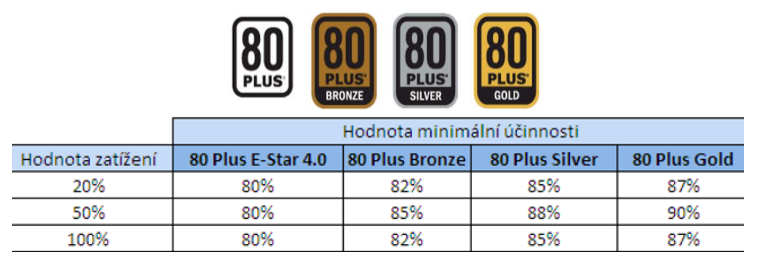
\includegraphics[scale=0.5]{sections/16_zdroj_BIOS_UEFI_boot/images/Screenshot 2024-08-23 002034.png}
\end{figure}

\subsubsection{PFC}
Power Factor Correction. Snaha zdroje o eliminaci rušení a výskyt vyšších harmonických složek, které deformují sinusový průběh.
\paragraph{Aktivní}
Realizace pomocí tranzistorů spolu s kondenzátory. Komplexní zapojení, kde je použita aktivní součástka. Nevýhoda muže být rušení od tranzistorů -> řešením je odrušovací kondenzátor
\paragraph{Pasivní}
Obsahuje pouze pasivní součástky (R, C, L)
Realizace pomocí cívky, která je na vstupu zdroje. Snaží se omezit špičky, které zdroj odebírá a tím upravuje sinusový průběh -> menší deformace

\subsubsection{Ochranné funkce zdroje}
\paragraph{OCP = Over Current Protect}
Ochrana při nadměrném proudu. Pokud je nastavená hodnota překročena, zdroj se vypne.

\paragraph{OVP = Over Voltage Protect}
Odpojí zdroj při vyšším napětí na větvi, než povoluje norma a limity.

\paragraph{OPP = Over Power Protect}
Odpojí zdroj, když je překročen maximální výkon zdroje daný výrobcem.

\paragraph{OTP = Over Temperature Protect}
Ochrana proti přehřátí zdroje. Při překročení maximální teploty se zdroj vypne.

\paragraph{SCP = Short Circuit Protection}
Ochrana při zkratu na sekundární části zdroje.


\subsection{BIOS a jeho součásti}
BIOS (Basic Input/Output System) je základní systémový software, který inicializuje hardware a zavádí operační systém. Obsahuje několik klíčových součástí:

\begin{itemize}
\item POST (Power-On Self Test)
\begin{itemize}
\item Kontrola základních funkčností hardwaru při spuštění počítače.
\item Zobrazí tabulku s nalezeným HW.
\item Nastaví rychlostní parametry HW podle hodnot uložených v CMOS.
\end{itemize}
\item Boot Loader
\begin{itemize}
\item Spouští operační systém z určeného zaváděcího zařízení.
\item Hledá ve vnější paměti boot sector a poté mu předá řízení. 
\end{itemize}
\item BIOS Setup Utility
\begin{itemize}
\item Umožňuje uživatelům konfigurovat hardware a systémové nastavení.
\item Toto nastavení pak býva uloženo v CMOS paměti.
\end{itemize}
\item BIOS Firmware
\begin{itemize}
\item Trvalý software uložený v ROM nebo flash paměti, který řídí základní operace počítače.
\end{itemize}
\end{itemize}

\subsection{UEFI a rozdíly v bootování}
UEFI (Unified Extensible Firmware Interface) je moderní náhrada za BIOS s pokročilými funkcemi a lepší podporou pro moderní hardware.

\begin{itemize}
\item Secure Boot
\begin{itemize}
\item Zajišťuje, že se zavádí pouze důvěryhodný software.
\end{itemize}
\item Podpora pro větší disky
\begin{itemize}
\item Umožňuje práci s disky většími než 2 TB.
\end{itemize}
\item Rychlejší bootování
\begin{itemize}
\item Zrychluje proces zavádění operačního systému.
\end{itemize}
\item Podpora 64 bit zařízení
\begin{itemize}
    \item BIOSY byly tradičně založen na 16 bit assembleru.
\end{itemize}
\end{itemize}

\paragraph{Fáze bootování}
\begin{itemize}
    \item PEI - Pre EFI Inicialization
    \begin{itemize}
        \item Aktivuje se CPU, pamět a čipová sad.
    \end{itemize}
    \item DXE - Driver Execution Enviroment
    \begin{itemize}
        \item Inicializace zbytku HW (paralelně).
    \end{itemize}
\end{itemize}

\subsection{CSM, Secure Boot, TPM}
\paragraph{CSM}
CSM (Compatibility Support Module) je součástí UEFI, která umožňuje kompatibilitu se staršími systémy a zařízeními podporujícími BIOS. Umožňuje použití starších operačních systémů a zařízení, která nejsou kompatibilní s UEFI.

\paragraph{Secure Boot}
Secure Boot je bezpečnostní standard vyvinutý v rámci UEFI specifikace, který zajišťuje, že počítač zavádí pouze software, který je důvěryhodný výrobcem zařízení. To pomáhá předcházet zavedení škodlivého softwaru při startu počítače.

\paragraph{TPM a princip fungování}
Trusted Platform Module (TPM) je specializovaný čip na základní desce, který poskytuje hardwarovou podporu pro bezpečnostní funkce. TPM ukládá šifrovací klíče, certifikáty a další bezpečnostní údaje. TPM zajišťuje integritu a důvěryhodnost systému a hraje klíčovou roli v moderních bezpečnostních funkcích, jako je BitLocker.

\subsection{Proces výběru a zavedení OS, instalace přes UEFI}
Při procesu zavádění operačního systému počítač provádí následující kroky:

\begin{itemize}
\item Inicializace hardwaru
\begin{itemize}
\item Systémový firmware inicializuje a kontroluje hardware.
\end{itemize}
\item Vyhledání zaváděcího zařízení
\begin{itemize}
\item Firmware hledá zaváděcí zařízení podle nastavení v BIOS/UEFI.
\end{itemize}
\item Zavedení boot loaderu
\begin{itemize}
\item Boot loader se načte z vybraného zaváděcího zařízení a spustí operační systém.
\end{itemize}
\item Předání kontroly operačnímu systému
\begin{itemize}
\item Po načtení základních komponent operačního systému se kontrola předává OS, který pokračuje v zavádění.
\end{itemize}
\end{itemize}

Instalace operačního systému přes UEFI se provádí následovně:

\begin{itemize}
\item Připravení instalačního média
\begin{itemize}
\item Vytvoření instalačního USB disku nebo DVD s podporou UEFI.
\end{itemize}
\item Konfigurace UEFI
\begin{itemize}
\item Přístup do UEFI nastavení a povolení UEFI bootování, případně vypnutí CSM.
\end{itemize}
\item Zavedení instalačního média
\begin{itemize}
\item Zavedení z instalačního média pomocí UEFI.
\end{itemize}
\item Instalace OS
\begin{itemize}
\item Postupování podle pokynů instalačního programu pro zavedení operačního systému.
\end{itemize}
\end{itemize}